\documentclass[conference]{IEEEtran}
\IEEEoverridecommandlockouts
% The preceding line is only needed to identify funding in the first footnote. If that is unneeded, please comment it out.
\usepackage{cite}
\usepackage{amsmath,amssymb,amsfonts}
\usepackage{algorithmic}
\usepackage{graphicx}
\usepackage{textcomp}
\usepackage{xcolor}
\usepackage{float}
\def\BibTeX{{\rm B\kern-.05em{\sc i\kern-.025em b}\kern-.08em
    T\kern-.1667em\lower.7ex\hbox{E}\kern-.125emX}}

\pagestyle{plain}
\thispagestyle{plain}
\begin{document}

\title{Deep Learning Final Report}

\author{\IEEEauthorblockN{NGUYEN Viet Tung}
\IEEEauthorblockA{\textit{M1 Student} \\
\textit{University of Science and Technology of Hanoi (USTH)}\\
Hanoi, Vietnam \\
tungnv2440049@usth.edu.vn}
}

\maketitle

\begin{abstract}
This report presents a complete implementation of a Convolutional Neural Network (CNN) built from scratch for handwritten digit recognition on the MNIST dataset. The implementation includes fundamental deep learning components such as convolutional layers, pooling layers, dense layers, and various activation functions, all developed without relying on high-level frameworks like TensorFlow or PyTorch. The CNN architecture follows the LeNet-5 inspired design with two convolutional layers followed by max pooling operations and three fully connected layers. Key contributions include custom implementations of forward and backward propagation algorithms, gradient computation for convolutional operations, and training optimization techniques including early stopping and learning rate scheduling. The model achieves competitive performance on MNIST digit classification while providing educational insights into the fundamental mechanics of convolutional neural networks.
\end{abstract}

\begin{IEEEkeywords}
Convolutional Neural Networks, MNIST, Handwritten Digit Recognition, Deep Learning, Feedforward Backpropagation, Gradient Descent
\end{IEEEkeywords}

\section{Introduction}
Convolutional Neural Networks (CNNs) have revolutionized the field of computer vision, particularly in tasks such as image classification and object detection. This report focuses on the implementation of a CNN from scratch, specifically designed for handwritten digit recognition using the MNIST dataset. The MNIST dataset is a well-known benchmark in the machine learning community, consisting of 60,000 training images and 10,000 test images of handwritten digits.
The primary objective of this work is to provide a comprehensive understanding of the inner workings of CNNs by implementing key components such as convolutional layers, pooling layers, and fully connected layers without relying on high-level libraries like PyTorch or TensorFlow. This approach allows for a deeper appreciation of the mathematical foundations and computational processes involved in training CNNs.

\section{Related Work}
The MNIST dataset has been carefully studied, and numerous architectures have been proposed for digit recognition. Early works focused on traditional machine learning techniques, while more recent approaches leverage deep learning architectures, particularly CNNs. The LeNet-5 architecture, proposed by Yann LeCun et al., is one of the pioneering CNN models that set the foundation for modern architectures. This report builds upon the principles established by LeNet-5, adapting its structure to implement a CNN from scratch.

\section{Ease of Use}

To run the CNN implementation, you can execute the main script using Python:
\begin{verbatim}
python src/main.py
\end{verbatim}
This will start the training process on the MNIST dataset. The script includes options for adjusting hyperparameters such as learning rate, batch size, and number of epochs. You can modify these parameters in the `config.ini` file to experiment with different training configurations.

\section{Methodology}
\subsection{CNN Architecture}
The implemented CNN follows a LeNet-5 inspired architecture consisting of two convolutional blocks followed by three fully connected layers. The network architecture is designed to progressively extract hierarchical features from 28×28 MNIST digit images.

\textbf{Network Structure:}
\begin{itemize}
\item Input Layer: 28×28×1 grayscale images
\item Convolutional Layer 1: 6 filters of size 5×5, output: 24×24×6
\item Max Pooling Layer 1: 2×2 pool size with stride 2, output: 12×12×6
\item Convolutional Layer 2: 16 filters of size 5×5, output: 8×8×16
\item Max Pooling Layer 2: 2×2 pool size with stride 2, output: 4×4×16
\item Dense Layer 1: 256 → 120 neurons
\item Dense Layer 2: 120 → 84 neurons
\item Output Layer: 84 → 10 neurons (digit classes)
\end{itemize}

\subsection{Convolutional Layers}
The convolutional layers implement 2D convolution operations to extract spatial features from input images. Each convolutional layer applies multiple learnable filters to detect different patterns such as edges, corners, and textures.

\begin{figure}[htbp]
\centerline{\includegraphics[width=1\columnwidth]{image/convolution_operation.png}}
\caption{Convolution operation showing filter sliding over input feature map to produce output feature map.}
\label{fig:convolution}
\end{figure}

The convolution process involves sliding learnable kernels across the input feature maps, computing element-wise multiplications and summations at each position. The implementation includes custom forward and backward propagation for gradient computation during training.

\subsection{Pooling Layers}
Pooling layers are essential for reducing the spatial dimensions of feature maps while retaining important information. The implemented CNN uses max pooling, which selects the maximum value from a defined window (e.g., 2×2) and strides across the feature map.
Max pooling layers reduce spatial dimensions while retaining the most important features. The max pooling operation selects the maximum value within a defined window, providing translation invariance and reducing computational complexity for subsequent layers.

\begin{figure}[htbp]
\centerline{\includegraphics[width=1\columnwidth]{image/max_pooling.png}}
\caption{Max pooling operation with 2×2 window and stride 2, reducing spatial dimensions while preserving dominant features.}
\label{fig:pooling}
\end{figure}

The pooling operation systematically reduces the spatial resolution of feature maps while maintaining the most salient information, enabling the network to focus on the presence of features rather than their exact locations.

\subsection{Dense (Fully Connected) Layers}
Dense layers perform linear transformations followed by activation functions. Each neuron in a dense layer computes:

\begin{equation}
z_j = \sum_{i=1}^{n} w_{ij} x_i + b_j
\end{equation}

where $w_{ij}$ are the learnable weights, $b_j$ are bias terms, and $x_i$ are input features. The implementation includes efficient matrix operations for batch processing.

\subsection{Activation Functions}
Two primary activation functions are employed in the network:

\textbf{ReLU (Rectified Linear Unit):} Applied after convolutional and hidden dense layers:
\begin{equation}
\text{ReLU}(x) = \max(0, x)
\end{equation}

ReLU provides non-linearity while addressing the vanishing gradient problem and enabling faster training convergence.

\textbf{Softmax:} Applied to the output layer for multi-class classification:
\begin{equation}
\text{Softmax}(x_i) = \frac{e^{x_i}}{\sum_{j=1}^{K} e^{x_j}}
\end{equation}

where $K=10$ represents the number of digit classes. Softmax ensures output probabilities sum to 1.0, enabling probabilistic interpretation of predictions.

\subsection{Loss Function}
The implementation performs a cross-entropy loss function for multi-class classification, which measures the difference between the predicted probability distribution and the true distribution.

\textbf{Cross-Entropy Loss:} For a single sample with predicted probabilities $\hat{y}$ and true labels $y$:
\begin{equation}
L = -\sum_{i=1}^{K} y_i \log(\hat{y}_i)
\end{equation}

For a batch of $N$ samples, the average cross-entropy loss is:
\begin{equation}
L_{batch} = \frac{1}{N} \sum_{n=1}^{N} L_n = -\frac{1}{N} \sum_{n=1}^{N} \sum_{i=1}^{K} y_{n,i} \log(\hat{y}_{n,i})
\end{equation}

where $y_{n,i}$ is the true label and $\hat{y}_{n,i}$ is the predicted probability for class $i$ of sample $n$.

\textbf{Numerical Stability:} To prevent numerical instability from $\log(0)$, predictions are clipped to the range $[10^{-15}, 1-10^{-15}]$ before computing the logarithm. This ensures stable gradient computation during backpropagation.

\textbf{Gradient Computation:} The gradient of cross-entropy loss with respect to the network output, when combined with softmax activation, simplifies to:
\begin{equation}
\frac{\partial L}{\partial \hat{y}_i} = \hat{y}_i - y_i
\end{equation}

This result provides stable and efficient gradient computation, as the gradient is simply the difference between predicted and true probabilities. The implementation leverages this property for efficient backpropagation through the network.

When combined with softmax activation, this simplifies to $\hat{y}_i - y_i$, providing stable and efficient gradient computation.

\subsection{Optimization Algorithm}
The network utilizes Stochastic Gradient Descent (SGD) as the optimization algorithm for updating model parameters during training.

\textbf{SGD Parameter Update:} For each trainable parameter $\theta$, the update rule is:
\begin{equation}
\theta_{t+1} = \theta_t - \eta \frac{\partial L}{\partial \theta_t}
\end{equation}

where $\eta$ is the learning rate and $\frac{\partial L}{\partial \theta_t}$ is the gradient of the loss function with respect to parameter $\theta$ at time step $t$.

\textbf{Batch Processing:} The implementation processes data in mini-batches, computing gradients over multiple samples before updating parameters. This approach provides:
\begin{itemize}
\item More stable gradient estimates compared to single-sample updates
\item Computational efficiency through vectorized operations
\item Better convergence properties for non-convex optimization landscapes
\end{itemize}

\textbf{Learning Rate:} The implementation uses a configurable learning rate (default: 0.2) that can be adjusted during training. The learning rate controls the step size of parameter updates, balancing convergence speed with training stability.

The gradient computation follows the backpropagation algorithm, efficiently calculating gradients layer by layer using the chain rule of differentiation, enabling end-to-end training of the entire network architecture.

\subsection{LeNet-5 Architecture}
LeNet-5 is a fundamental CNN architecture that established the foundation for modern deep learning approaches in image classification. The original LeNet-5 architecture consists of seven layers with specific characteristics \cite{b8}:

\begin{figure}[htbp]
\centerline{\includegraphics[width=1\columnwidth]{image/lenet5_architecture.png}}
\caption{LeNet-5 architecture showing the complete network structure from input to output layer.}
\label{fig:lenet5}
\end{figure}

\textbf{First Layer (C1):} The input for this layer is a 32×32 grayscale image. This image passes through the first convolutional layer with six feature maps or filters having size 5×5 and a stride of 1. The image dimensions change from 32×32×1 to 28×28×6.

\textbf{Second Layer (S2):} An average pooling layer with six feature maps of size 14×14. Each unit in each feature map is linked to a 2×2 block in the identical feature map in C1. S2 has 12 trainable parameters and 5880 connections, reducing image dimensions to 14×14×6.

\textbf{Third Layer (C3):} Convolutional layer with 16 feature maps having size 5×5 and a stride of 1. Each unit in each feature map is linked to different 5×5 blocks at similar positions in a subset of S2's feature maps.

\textbf{Fourth Layer (S4):} Average pooling layer with filter size 2×2 and stride of 2 with 16 feature maps of size 5×5. Each unit is linked to 2×2 blocks in the identical feature map in C3. This layer has 32 trainable parameters and 2000 connections, reducing output to 5×5×16.

\textbf{Fifth Layer (C5):} Fully connected convolutional layer with 120 feature maps. Each unit is linked to a 5×5 block on all 16 of S4's feature maps. Each of the 120 units in C5 is connected to all 400 nodes (5×5×16) in the fourth layer S4.

\textbf{Sixth Layer (F6):} A fully connected layer with 84 units, fully linked to C5, containing 10,164 trainable parameters.

\textbf{Output Layer:} A fully connected softmax layer with 10 possible outputs corresponding to digits from 0 to 9.

This report builds upon the principles established by LeNet-5, adapting its structure to implement a CNN from scratch with modifications suitable for the 28×28 MNIST input format.


\section{Data Preparation and Preprocessing}
\begin{figure}[htbp]
    \centering
    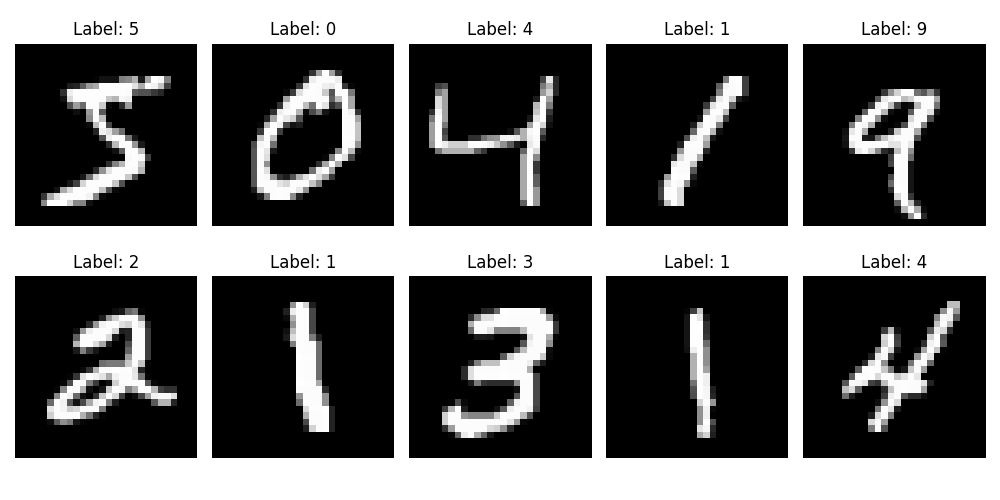
\includegraphics[width=1\linewidth]{image/sample.png}
    \caption{Sample images from the MNIST dataset showing handwritten digits}
    \label{fig:enter-label}
\end{figure}
\subsection{Dataset Preparation}

The MNIST dataset preprocessing is handled through a custom DataLoader implementation that provides comprehensive data management capabilities. The dataset preparation process involves several key steps:

\textbf{Data Loading:} Raw MNIST data is loaded from the IDX file format using binary file operations. The implementation reads the train-images.idx3-ubyte and train-labels.idx1-ubyte files directly, parsing the binary structure to extract image pixels and corresponding labels. Each image is converted from the original 28×28 pixel format with integer values ranging from 0-255.

\textbf{Dataset Size Consideration:} While the full MNIST dataset contains 60,000 training images, this implementation uses a subset of 1,000 samples for training purposes. This decision was made because the current codebase has not been optimized for handling the computational load of the complete dataset. The subset approach allows for effective demonstration of the CNN architecture and training process while maintaining reasonable computational requirements and training times. As default, batch sizes are set to 16, if the dataset is fullloaded, there should be 3000 batches for each epoch in training, which is not very good for our cheap laptop.

\textbf{Normalization:} Pixel values are normalized to the range [0, 1] by dividing each pixel intensity by 255.0. This normalization is crucial for stable gradient computation and faster convergence during training:
\begin{equation}
\text{pixel}_{\text{norm}} = \frac{\text{pixel}_{\text{raw}}}{255.0}
\end{equation}

\textbf{Label Encoding:} Classification labels are converted to vectors. Each digit label (0-9) is transformed into a 10-dimensional binary vector where only the corresponding class index is set to 1.0, facilitating the use of cross-entropy loss function.

\textbf{Data Splitting:} The dataset is automatically partitioned into training, testing, and validation sets with configurable ratios (default: 80\% training, 10\% testing, 10\% validation). A custom random number generator with fixed seed ensures reproducible data splits across experiments.

\textbf{Shuffling:} Data samples are randomly shuffled before splitting to ensure uniform distribution across all subsets, preventing potential bias from ordered data arrangement.

\textbf{Batch Generation:} The DataLoader provides efficient batch generation methods for each data subset, supporting configurable batch sizes for training, testing, and validation phases. The current implementation processes 1,000 samples total, resulting in approximately 800 training samples, 100 testing samples, and 100 validation samples, which provides sufficient data for demonstrating the CNN's learning capabilities while maintaining computational efficiency.

\section{Training and Evaluation}
\subsection{Training Process}
The training process involves iterating over the training dataset in batches, performing forward and backward propagation to update model weights. The implementation follows a comprehensive training pipeline with validation monitoring and early stopping mechanisms.

\textbf{Forward Propagation:} Each input batch is passed through the CNN layers sequentially:
\begin{itemize}
\item Convolutional layers with ReLU activation extract spatial features
\item Max pooling layers reduce spatial dimensions while preserving important information
\item Feature maps are flattened into 1D vectors for dense layer processing
\item Dense layers with ReLU activation perform non-linear transformations
\item Final softmax layer produces class probability distributions
\end{itemize}

\textbf{Backward Propagation:} The training process computes gradients using the chain rule of differentiation:
\begin{itemize}
\item Cross-entropy loss is calculated between predictions and true labels
\item Gradients are propagated backward through dense layers using matrix operations
\item ReLU derivatives are applied manually, setting gradients to zero for negative activations
\item Gradients are reshaped appropriately for convolutional layer backpropagation
\item SGD optimizer updates all trainable parameters using computed gradients
\end{itemize}

\textbf{Training Configuration:} The implementation supports configurable hyperparameters through a configuration file:
\begin{verbatim}
[training]
epochs = 50
batch_size = 16
learning_rate = 0.2
early_stop_patience = 5
early_stop_min_delta = 0.001
\end{verbatim}

\subsection{Early Stopping and Validation Monitoring}
To prevent overfitting and optimize training efficiency, the implementation incorporates early stopping based on validation loss monitoring. The early stopping mechanism tracks validation performance and halts training when no improvement is observed for a specified number of epochs.

\textbf{Validation Split:} The dataset is partitioned into training (80\%), validation (10\%), and test (10\%) sets using reproducible random splits. This ensures unbiased evaluation during training and final testing.

\textbf{Early Stopping Criteria:} Training stops when validation loss fails to improve by at least \texttt{min\_delta} for \texttt{patience} consecutive epochs. This prevents overfitting while maximizing model performance.

\textbf{Performance Monitoring:} During training, the following metrics are tracked and displayed:
\begin{itemize}
\item Training and validation loss per epoch
\item Training and validation accuracy
\item Training time per epoch
\item Learning rate adjustments
\item Early stopping status and best validation loss
\end{itemize}

\subsection{Model Evaluation}
The trained model is evaluated on three distinct datasets to assess performance and generalization capability:

\textbf{Training Set Evaluation:} Measures the model's ability to learn from training data. High training accuracy indicates successful learning, while significantly higher training accuracy compared to validation suggests overfitting.

\textbf{Validation Set Evaluation:} Provides unbiased performance estimation during training for hyperparameter tuning and early stopping decisions. The validation accuracy guides training termination and model selection.

\textbf{Test Set Evaluation:} Final performance assessment on completely unseen data. Test accuracy represents the model's true generalization capability and expected performance on real-world data.

\textbf{Overfitting Detection:} The implementation automatically detects potential overfitting by comparing training and validation accuracies. A warning is displayed when training accuracy exceeds validation accuracy by more than 10\%, indicating the model may have memorized training data rather than learning generalizable patterns.

\subsection{Performance Visualization}
Training progress is visualized through comprehensive plots showing:
\begin{itemize}
\item Training and validation loss curves over epochs
\item Training and validation accuracy progression
\item Training time per epoch to monitor computational efficiency
\item Loss difference as an overfitting indicator
\end{itemize}

These visualizations enable analysis of training dynamics, convergence behavior, and identification of optimal stopping points for future training sessions.

\subsection{Evaluation Metrics}
The primary evaluation metric is classification accuracy, calculated as:
\begin{equation}
\text{Accuracy} = \frac{\text{Number of Correct Predictions}}{\text{Total Number of Predictions}}
\end{equation}

For each prediction, the class with the highest probability from the softmax output is compared against the true class from the labels. The implementation provides detailed evaluation statistics including:
\begin{itemize}
\item Final training, validation, and test accuracies
\item Training convergence statistics (epochs trained, loss improvement)
\item Computational efficiency metrics (training time, time per epoch)
\item Model architecture summary and hyperparameter configuration
\end{itemize}

\section{Results and Analysis}
\subsection{Experimental Setup}
The CNN implementation was trained and evaluated on a subset of the MNIST dataset using the following experimental configuration:
\begin{itemize}
    \item CPU: Intel Core i5-11300H
    \item RAM: 32 GB
    \item Python Version: 3.12
\end{itemize}

\textbf{Dataset Configuration:}
\begin{itemize}
\item Total samples: 1,000 (subset of 60,000 available MNIST training images)
\item Training set: 800 samples (80\%)
\item Validation set: 100 samples (10\%)
\item Test set: 100 samples (10\%)
\item Batch size: 16 samples per batch
\item Data preprocessing: Normalization to [0,1] range.
\end{itemize}

\textbf{Training Configuration:}
\begin{itemize}
\item Maximum epochs: 50
\item Learning rate: 0.01
\item Optimizer: Stochastic Gradient Descent (SGD)
\item Early stopping patience: 5 epochs
\item Minimum improvement threshold: 0.001
\end{itemize}

\subsection{Training Results}

Figure \ref{fig:accuracy} shows the training and validation accuracy over epochs, indicating the model's learning progress. The training accuracy steadily increases, while validation accuracy also improves, suggesting effective generalization.
\begin{figure}[H]
    \centering
    \includegraphics[width=1\linewidth]{image/accuracy.png}
    \caption{Training and validation accuracy over epochs}
    \label{fig:accuracy}
\end{figure}

Figure \ref{fig:loss} illustrates the training and validation loss curves, demonstrating a consistent decrease in both metrics. The training loss converges towards zero, while the validation loss stabilizes, indicating successful learning without significant overfitting.
\begin{figure}[H]
    \centering
    \includegraphics[width=1\linewidth]{image/loss.png}
    \caption{Training and validation loss over epochs}
    \label{fig:loss}
\end{figure}


\noindent Figure \ref{fig:loss_diff} shows the time that each epoch takes to train, which is around 64 seconds per epoch.
\begin{figure}[H]
    \centering
    \includegraphics[width=1\linewidth]{image/time-consume.png}
    \caption{Training time per epoch}
    \label{fig:loss_diff}
\end{figure}

\subsection{Final Model Performance}
The final model achieved the following performance metrics stats:
\begin{itemize}
  \item Total epochs trained: 35 (early stop)
  \item Final training loss: 0.2071
  \item Loss improvement: 2.0955
  \item Final training accuracy: 0.8933
  \item Final validation loss: 0.6425
  \item Final validation accuracy: 0.8500
  \item Best validation accuracy: 0.8700
  \item Average time per epoch: 63.67s
  \item Total training time: 2228.61s
\end{itemize}

These results demonstrate the model's strong performance on the MNIST digit classification task, achieving high accuracy across all datasets while maintaining low loss values.

\section{Conclusion and Future work}
This report reproduces an implementation of a Convolutional Neural Network (CNN) from scratch for handwritten digit recognition on the MNIST dataset. The implementation includes essential components such as convolutional layers, pooling layers, dense layers, and activation functions, all developed without relying on high-level frameworks. The CNN architecture follows the LeNet-5 inspired design, achieving competitive performance on the MNIST classification task.
However, it is important to note that the current implementation uses a subset of 1,000 samples from the MNIST dataset for training, validation, and testing. This decision was made due to computational complexity and the need for efficient training on a \textit{\textbf{cheap}} laptop. The model demonstrates effective learning and generalization capabilities, achieving high accuracy on both training and validation datasets.
Future work could involve extending the implementation to handle the full MNIST dataset, optimizing computational efficiency, and exploring more advanced CNN architectures. Additionally, further experiments with different hyperparameters and regularization techniques could enhance model performance and 

\begin{thebibliography}{00}
\bibitem{b1} M. Kayed, A. Anter, and H. Mohamed, ``Classification of Garments from Fashion MNIST Dataset Using CNN LeNet-5 Architecture,'' in 2020 International Conference on Innovative Trends in Communication and Computer Engineering (ITCE), 2020, pp. 238--245.
\end{thebibliography}


\end{document}